%%%%%%%%%%%%%%%%%%%%%%%%%%%%%%%%%%%%%%%%%
% Friggeri Resume/CV
% XeLaTeX Template
% Version 1.2 (3/5/15)
%
% This template has been downloaded from:
% http://www.LaTeXTemplates.com
%
% Original author:
% Adrien Friggeri (adrien@friggeri.net)
% https://github.com/afriggeri/CV
%
% License:
% CC BY-NC-SA 3.0 (http://creativecommons.org/licenses/by-nc-sa/3.0/)
%
% Important notes:
% This template needs to be compiled with XeLaTeX and the bibliography, if used,
% needs to be compiled with biber rather than bibtex.
%
%%%%%%%%%%%%%%%%%%%%%%%%%%%%%%%%%%%%%%%%%
% Modified 2017 by:
% Andreas Offenhaeuser (http://anoff.io)
%%%%%%%%%%%%%%%%%%%%%%%%%%%%%%%%%%%%%%%%%

\documentclass[]{friggeri-cv} % Add 'print' as an option into the square bracket to remove colors from this template for printing

\begin{document}

\header{andreas}{of\/fenhaeuser}{cloud solution architect}{git:COMMITID}

%----------------------------------------------------------------------------------------
%	SIDEBAR SECTION
%----------------------------------------------------------------------------------------

\begin{aside} % In the aside, each new line forces a line break
\section{\color{red}contact}
Stuttgart, Germany
\href{mailto:offenhaeuser@gmail.com}{offenhaeuser@gmail.com}
\graytitle{web}{\href{http://www.anoff.io}{anoff.io}}
\graytitle{github}{\href{http://www.github.com/anoff}{gh/anoff}}
\graytitle{twitter}{\href{http://twitter.com/an0xff}{@an0xff}}
\section{\color{purple}languages}
\graytitle{native}{german}
\graytitle{professional}{english}
\graytitle{beginner}{japenese, french}
\section{\color{green}craftsmanship}
{\color{red} $\varheartsuit$} Node.js, JavaScript
Python, Matlab
bash, C
software design
system understanding
agile methods
continuous deployment
\hfill
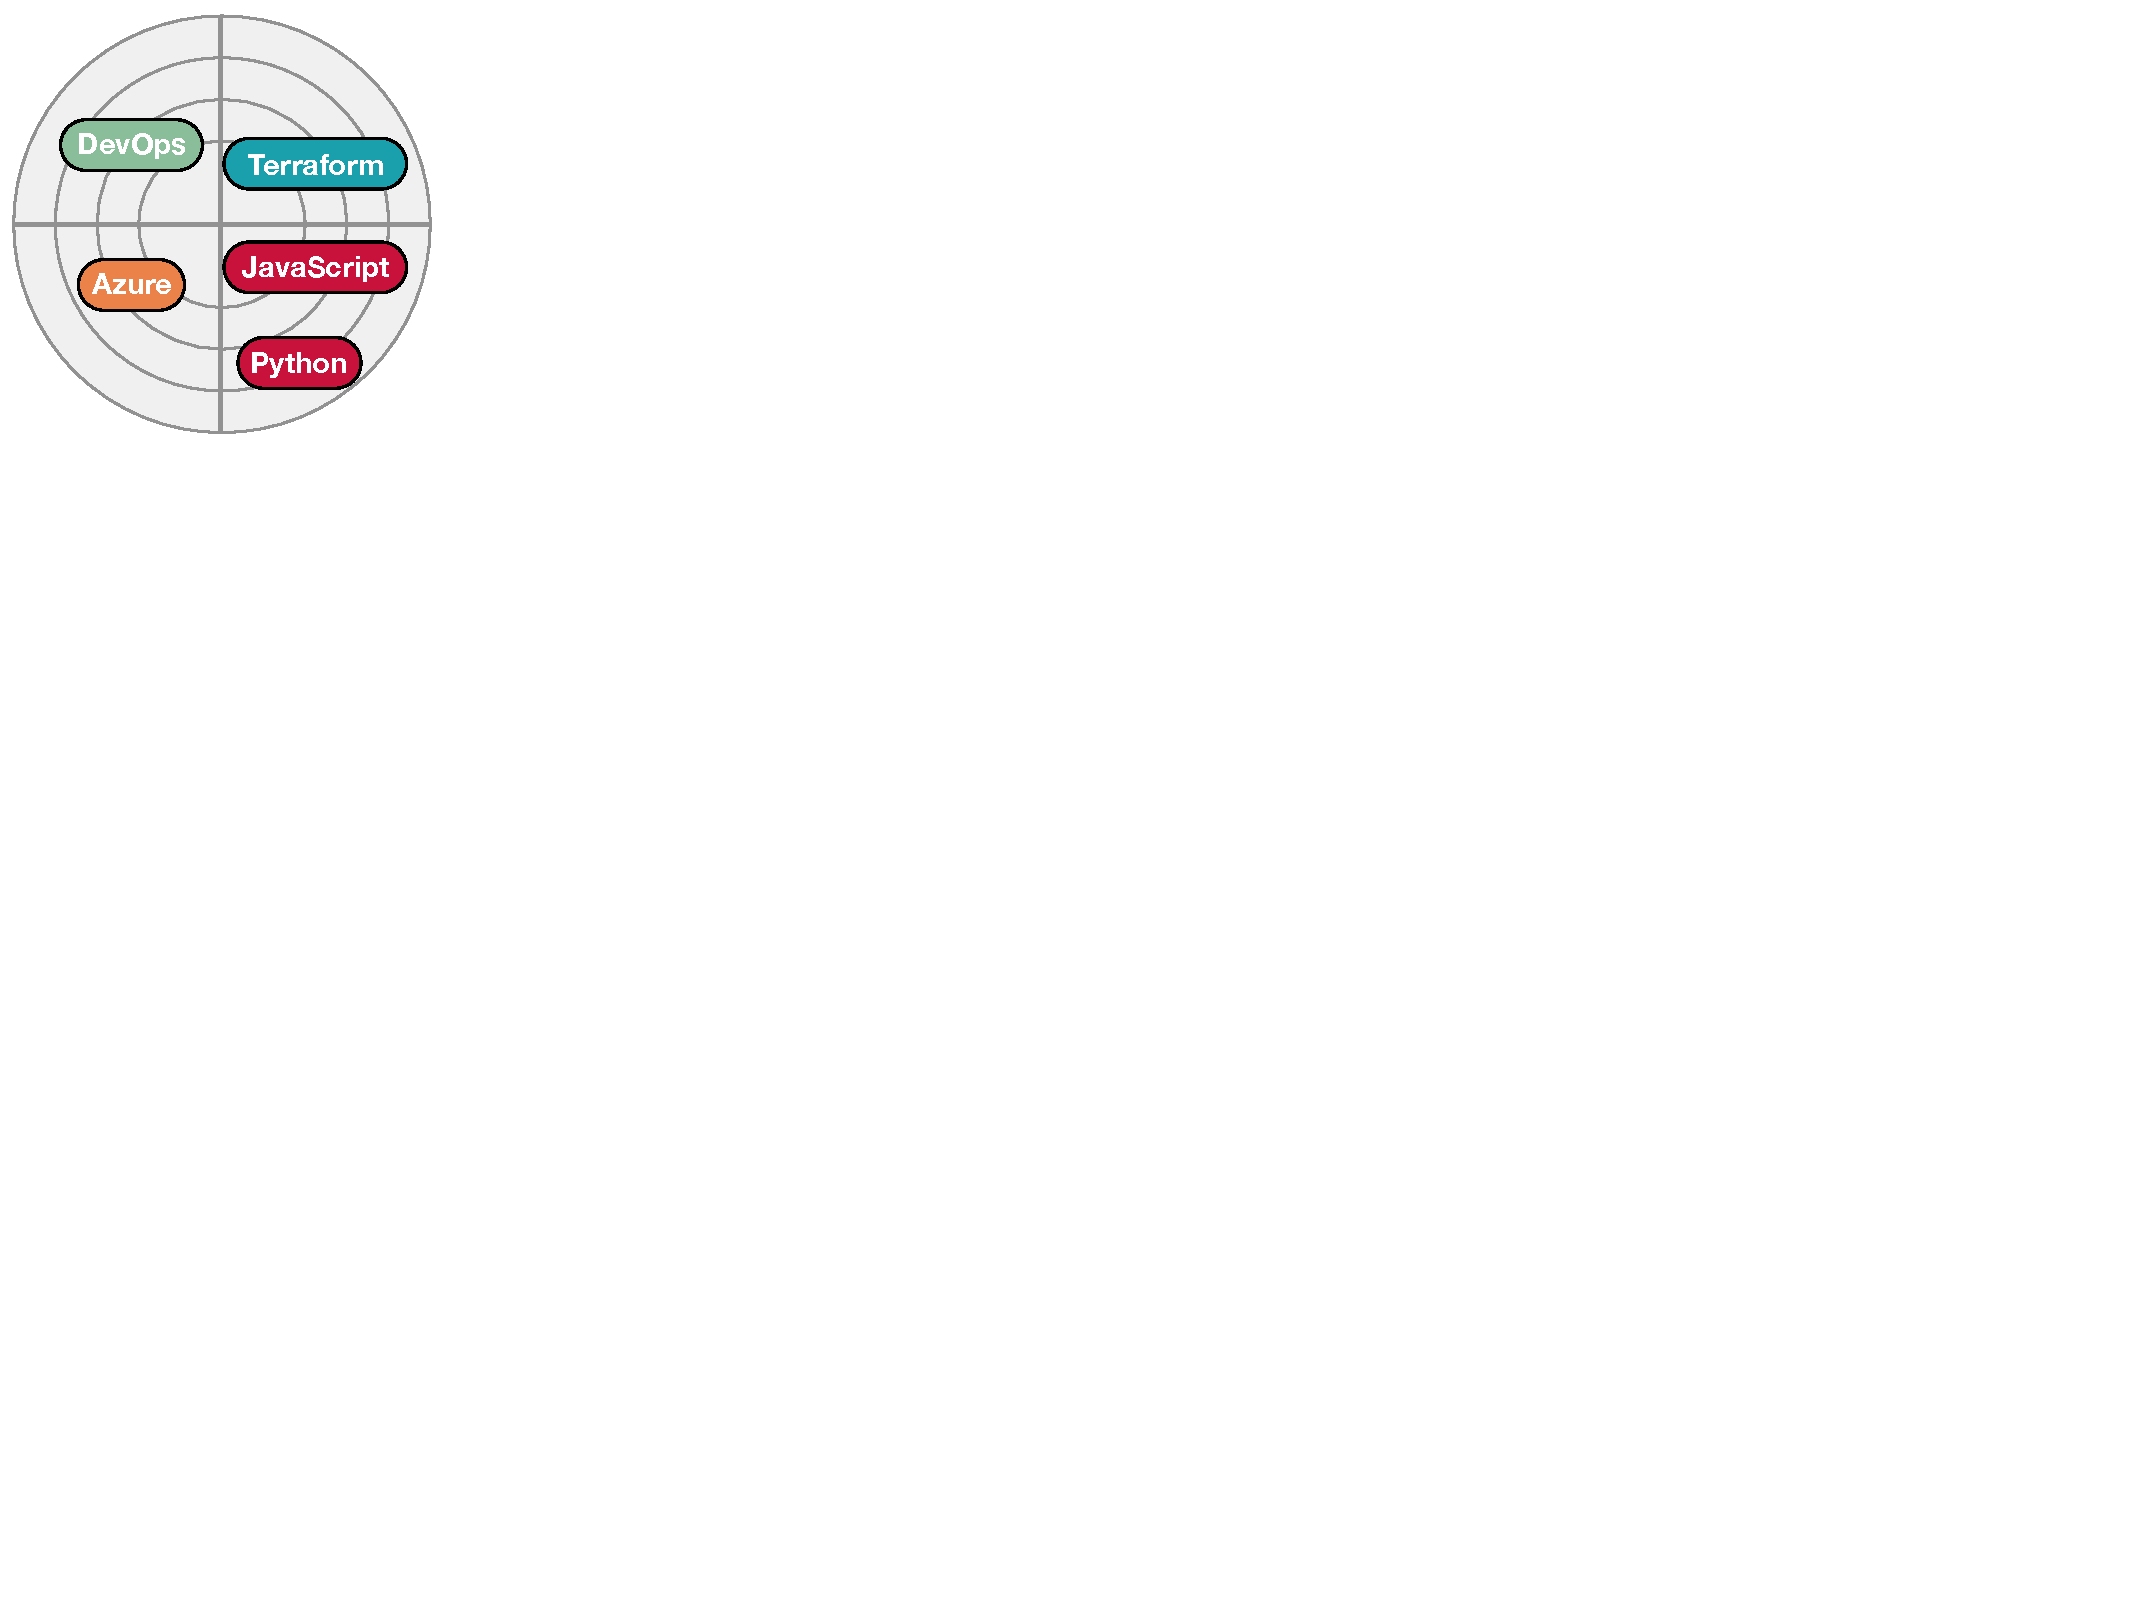
\includegraphics[clip, width=0.8\textwidth, trim=0cm 19cm 28cm 0cm]{radar.pdf}
\textit{Visit \href{https://tech.anoff.io}{tech.anoff.io} for my personal technology radar}
\section{\color{blue}domains}
cloud solutions
automotive systems
robotics
\end{aside}

%----------------------------------------------------------------------------------------
%	WORK EXPERIENCE SECTION
%----------------------------------------------------------------------------------------

\section{\color{orange}experience}

\begin{entrylist}

%------------------------------------------------

\entry
{2016--}
{Solution Architect}
{Robert Bosch GmbH, Stuttgart DE}
{Responsible for backend architecture of connected vehicle services. This includes designing cloud solutions according to domain driven principles as well as implementing features in our SCRUM team. I am familiar working with the Cloudfoundry PaaS stack for Microservices as well as designing and implementing Javascript based solutions on Microsoft Azure serverless components. Investing heavility into automation with Terraform my daily real job description lies somewhere between solution architect and software engineer.

\skills{aquired skills}{Node.js, OSS compliance, solution architecture, Cloudfoundry, Azure, Infrastructure as Code}
}
\end{entrylist}
\begin{entrylist}
\entry
{2014--2016}
{Backend developer connected vehicle}
{Robert Bosch GmbH, Stuttgart DE}
{Starting 2014 I was responsible for designing and developing a prototype system for a connected vehicle. It was a fullstack job where I was resonsible to manage a team of up to five to set up servers, develop backend \& frontend as well as the vehicle communication. In 2015 the project left prototype state and a larger team was built up to develop the system with a more mature state. I was involved in selecting the team members and defining the development processes.

\skills{aquired skills}{Node.js, AngularJS, Docker, project management}
}
\end{entrylist}
\begin{entrylist}
\entry
{2012--2014}
{Function developer for driver monitoring}
{Robert Bosch GmbH, Stuttgart DE}
{Following my experiences as a test manager I switched sides and started developing algorithms for driver monitoring. This involved handling of larger data sets within Matlab and building a simulation environment capable of handling multiple thousands kilometers of test data to evaluate algorithm performance. With changing algorithms it was also necessary to develop new scoring functions. Development of series code was done according to automotive SPICE requirements. In 2013 I was also leading a 8 month project study with a german automotive OEM to identify the potential of new driver monitoring functions.

\skills{aquired skills}{statistics, data handling, requirements engineering, change management, Matlab, project management, ASPICE}
}
\end{entrylist}
\begin{entrylist}
\entry
{2010--2012}
{Test manager for driver monitoring software}
{Robert Bosch GmbH, Stuttgart DE}
{Responsible for planning automotive software tests from unit to system level. On system level I was also responsible for designing and implementing the test environment for hardware in the loop simulation of a automotive ECU. This had to be integrated into existing quality frameworks and comply with functional safety according to ISO26262.

\skills{aquired skills}{systems engineering, project management, vehicle communication (CAN/FlexRay), test methodology, CANoe, VBA}
}
\end{entrylist}
\begin{entrylist}
\entry
{2009}
{Internship - motorcycle hydraulic simulation}
{Bosch Corporation, Yokohama JP}
{As part of my studies I accomplished a six months internship in Japan. My task was to create a simulation environment for motorcycle ABS systems. I had to collect requirements from different engineers, research motorcycle hydraulics and then develop a simulation with a user interface. The development was done in Matlab \& Matlab Simulink.

\skills{aquired skills}{Matlab, systems engineering, fluid physics, GUI design}
}
\end{entrylist}

%----------------------------------------------------------------------------------------
%	EDUCATION SECTION
%----------------------------------------------------------------------------------------
\section{\color{blue}education}

\begin{entrylist}

\entry
{2017--2018}
{Artificial Intelligence {\normalfont Nanodegree}}
{Udacity}
{Pursuing a deeper understanding of AI fundamentals I chose to join the nanodegree program and improve my knowledge in game agents, probabilistics and other AI methods. In my third term I specialized in computer vision methods.}

\entry
{2017}
{Deep Learning {\normalfont Foundation Nanodegree}}
{Udacity}
{Intrigued and fascinated by the advances of artificial intelligence I wanted to get a deeper understanding of the topic and joined the class of Udacitys newly introduced Deep Learning program. Within the course I worked on several projects ranging from image recognition to generative networks.}

\entry
{2007--2010}
{Bachelor {\normalfont of Engineering}, 1.3}
{Hochschule Heilbronn, DE}
{With a grant from Bosch I studied different fields of mechatronics and microsystems engineering. For my thesis I analyzed the influence of advanced driver assistance systems on steering based driver monitoring systems. The main focus was on data analytics and combined Matlab with scientific knowledge.
}

\entry
{2005--2007}
{Vocational training}
{Robert Bosch GmbH, DE}
{During my vocational training I learned the basics of engineering and how they relate to the physical world. The broad scope of topics covered in mechatronics also quickly made me realize my love for programming over the other possible fields in engineering.
}
\end{entrylist}

%----------------------------------------------------------------------------------------
%	INTERESTS SECTION
%----------------------------------------------------------------------------------------

\section{\color{green}interests}
\begin{itemize}
\item learning new technologies (blockchain, artificial intelligence, robotics, deep learning)
\item share \& exchange knowledge on meetups/confs
\item skiing, biking, diving
\item cooking
\end{itemize}


\section{\color{purple}side projects}
  \textit{A selection of my OSS projects. For more see my \href{http://www.github.com/anoff}{GitHub profile} or \href{http://anoff.io}{website}.}
  
  \project{plantbuddy}{https://plantbuddy.site}{A fullstack IoT solution to monitor plants. ESP8266 chip with device connectivity, serverless backend and a web frontend}
  
  \project{demo one}{https://github.com/anoff/demo-one}{3D graphics demo written in C++}
  
  \project{deep emoji gan}{https://github.com/anoff/deep-emoji-gan}{An approach to use DCGAN neural networks to generate emojis}

  \project{techradar}{https://radar-demo.anoff.io}{Framework to build custom technology radars, inspired by the \href{https://www.thoughtworks.com/radar}{Thoughtworks Radar}}

  \project{microllaborators}{https://github.com/anoff/microllaborators}{A distributed web app with serverless backend and augmented reality features.}

  \project{serial-io}{https://github.com/anoff/serial-io}{Node.js library to send serial commands with a promise based API}
\end{document}
